\documentclass[letterpaper]{article}
\usepackage{aaai}
\usepackage{times}
\usepackage{helvet}
\usepackage{courier}
\usepackage{amsmath,amssymb,amsthm,fullpage,mathtools}
\usepackage{mathtools}
\usepackage[english]{babel}
\usepackage{graphicx}
\usepackage{fontspec}
\usepackage{newunicodechar}
\usepackage{multicol}
\usepackage[margin={1.5cm,1.5cm}]{geometry}
\usepackage{hyperref}
\setlength{\pdfpagewidth}{8.5in}
\setlength{\pdfpageheight}{11in}
% \pdfinfo{
% /Title (Predicting the Efficiency of Organic Photovoltaics)
% /Author (Kevin K. Eskici, Luis A. Perez, Aidi Zhang)}
\setcounter{secnumdepth}{0}

% we want to adjust the seperationg between columns
\setlength{\columnsep}{1cm}

\title{Predicting the Efficiency 
of Organic Photovoltaics: \\
Computationally Efficient Machine Learning Methods
}
\author{Kevin Eskici\thanks{keskici@college.harvard.edu}, Luis A. Perez\thanks{luisperez@college.harvard.edu}, Aidi Zhang\thanks{aidizhang@college.harvard.edu} \\
Kaggle Team: cacheMoney \\
Computer Science, Harvard University}

\date{\today} 

\begin{document}

\maketitle

\begin{abstract}
\begin{quote}
In this paper, we take molecular data from the Harvard Clean Energy Project to train a statistical model that predicts HOMO-LUMO energy gap values for a set of test data. We discuss various machine learning models, including Ordinary Least Squares Regression, Ridge Regression, Lasso, K-Nearest Neighbors and Neural Networks, and experimental results are presented to indicate relative performances of these models. We also explore various feature space representations, including different ways of implementing feature extraction and selection to best improve prediction. We conclude with the importance of feature selection, especially when dealing with unstructured data, over model selection. Different models improved RMS by less that $0.01$, while extensive feature selection and extraction improved RMS by more than $0.1$.
\end{quote}
\end{abstract}

\section{Introduction}
% Information on the problem we're tackling
Machine learning on molecules is a unique and interesting problem because of the complexity of molecular structure. Whereas quantum calculations and empirical research might take days to derive desired properties on a single problem \footnote{As described in the practical handout.}, machine learning techniques present a faster and more efficient way of predicting molecular properties.\\

\noindent Finding a computationally efficient method of predicting the HUMO/LUMO gap, for example, could lead to developments in organic photo-voltaics, potentially reducing the energy costs of the nation through increased efficiency of solar panels. However, a majority of standard regression techniques model target variables given real-valued input predictor variables, and it is not immediately clear how best to represent entire molecules as inputs. Even if an accurate representation is found, the question remains of what features from our representation are the best predictors. Finally, even after the features are selected and modified in a way suitable for capturing accurate predictions, the model of problem selection and optimization remains.\\

\noindent In this paper, we consider the pros and cons of various representations of molecules. To start, we were given the standard 256-bit bit-vector extracted from RDKit Morgan Fingerprint \footnote{Standard Chemistry library for the Python}. The Morgan FingerPrint \footnote{\href{http://rdkit.org/UGM/2012/Landrum_RDKit_UGM.Fingerprints.Final.pptx.pdf}{Fingerprints in RDKit}} of a  but an important improvement involved choosing a better feature space. We will also consider the dilemma of feature selection vs feature extraction, as well as the computational consideration associated with each.

\section{Methodology}
% Information on the computational setup
 For computations, and in particular new feature extraction as discussed later in the text, we utilized three separate machines, shown out in Table \ref{tab:computers}.
 
\begin{table}
\begin{center}
    \begin{tabular}{ | p{2cm} | p{1cm} | p{2cm} | p{2cm} |}
    \hline
    Machine \# & CPU Model & Memory Used/Total & Cores Used/Total \\ \hline
    1 & Intel Core i5 & 4GB/4GB + 2GB Swap & 2/4 \\ \hline
    2 & Intel Core i7 & 8GB/8GB + 27GB Swap & 3/4 \\ \hline
    3 & Intel Core i7 & 10GB/10GB + 2GB Swap & 3/4 \\
    \hline
    \end{tabular}
    \caption{Machine processing power used for feature extraction and model training.}
    \label{tab:computers}
\end{center}
\end{table}
 
\noindent The machines were placed into an ad-hoc distributed system. We accomplished this be separating both the original training set and test sets into smaller chunks. The training sets consists of 1M feature, so we sub-divided it into 20 chunks, each of 50K data points. This was particularly helpful when generating new features because feature generation on a static set of molecules can be calculated in parallel. The 50K figure was selected after multiple trials on different sizes, noting that as the number of molecules increased, processing of the data seemed to grow at some non-linear factor ($\Omega(n^1+\epsilon)$ for some $\epsilon > 0$). The theory behind this, as it stands, is related to Python's own memory management \footnote{\href{https://docs.python.org/2/c-api/memory.html}{Python Memory Management in Detail}}.\\ 
\\

\noindent We suspect that after a certain number of gigabytes of physical memory are utilized by a single object, part of the object is placed into swap space. This significantly slows down processing. However, by maintaining a relatively small data-set loaded for each iPython kernel, we maintained a clean system. Each iPython kernel ran in a separate core on the above machines, leading to the calculation of 400K data points per cycle. Each cycle took around \~30 minutes for data extraction and ~10min for data prediction. \\
\\
\noindent We note, however, that the training needed to take place on the entire set. Loading this into memory for the original 256-bit vector proved possible, but as we expanded our features set, the problem posed was significant. The resolution to this problem further later in the paper. As for the testing set, a similar approach was taken for feature extraction. With around 800K data points, the total time to generate the features entered the hours range.

\noindent As hinted, the above calculations were performed using iPython, and in particular, iPython notebook. The primary off-the-shelve libraries used for computation purposes included both rdkit, mostly for feature extraction, and scikit-learn for the purposes of training our models, discussed below.

% LINEAR REGRESSION OLS
\subsection{Linear Regression}
In the simplest linear regression approach, we consider linear basis function models that minimizes the sum-of-squares error function. To determine whether a regression function $f(x) = x^{T} \omega$ is a good candidate, we have to ask whether $\omega$ is close to the true $\omega$, as well as whether $f(x)$ will fit future observations well. Good estimators should, on average, have small prediction errors; the prediction error at a specific input value $x$ is given by:

\begin{center}
$$ E_D [ (y(x;D) - h(x))^2 ]$$
$$= E_D[ [y(x;D)] - h(x)]^2 $$
$$+ E_D [ (y(x;D)-E_D[y(x;D)])^2 ] $$
\end{center} 

\noindent The first term and second term point to the bias and variance of the regression respectively. Introducing a little bias in our estimate of $\omega$ might lead to a substantial decrease in variance of our linear coefficients, and hence a substantial decrease in prediction error.\\
\\
\noindent We can write the error function rewritten in matrix form as such:

\begin{equation}
\begin{split}
E(\omega) &= arg \min_{\omega} \frac{1}{2} \sum_{i=0}^m \left( y_i - \omega_0 - \sum_{j=1}^{n} \omega_j x_{ij} \right)^2 \\
&= arg \min_{\omega} \frac{1}{2} (y - X\omega)^{T} (y - X\omega)
\end{split}
\end{equation}

\noindent We can obtain a closed-form solution by differentiating E with respect to $\omega$, obtaining:

$$\frac{\partial E}{\partial \omega} = X^{T}(y-X\omega) = 0 \Rightarrow \omega_{opt} = (X^{T}X)^{-1} X^{T}y$$

\noindent However, Ordinary Least Squares linear regression is susceptible to over-fitting the model \footnote{\href{http://www.jdl.ac.cn/user/hchang/course_staffs/02_overfitting\%20and\%20model\%20selection.pdf}{Over-fitting and model selection}}. Subsequently, we explore Ridge and Lasso Regression, both of which seek to alleviate the consequences of multi-collinearity among predictor variables. 


% RIDGE REGRESSION
\subsection{Ridge Regression}
If unconstrained, our regression coefficients might blow up and be susceptible to high variance \footnote{\href{http://www.stat.cmu.edu/~ryantibs/datamining/lectures/16-modr1.pdf}{Data mining lecture on ridge regression}}. For example, when variables are highly correlated, a large coefficient in one variable might be counteracted with a large coefficient in another, which is negatively correlated with the former.\\ 
\\
\noindent We want to use regularization to put an upper threshold on the values taken by coefficients. Regularization is a simple way to avoid over-fitting and often improves the prediction accuracy on new data. Our new residual sum of squares error function has an addition of a penalty term on coefficients that looks like this:

$$E(\omega) = \frac{1}{2} \sum_{n=1}^N (y(x_n,w) - t_n)^2 + \frac{\lambda}{2} \lVert w \rVert ^2$$

\noindent {\bf Derivation of Ridge Regression}\\
Similar to how we made the conversion to matrix representation and solved for the closed form solution for the Ordinary Least Squares approach above, we get

\begin{equation}
\begin{split}
E(\omega) &= arg \min_{\omega} \frac{1}{2} (y - X\omega)^{T} (y - X\omega) + \frac{\lambda}{2} \omega^{T} \omega \\
& \Rightarrow \frac{\partial E}{\partial \omega} = X^{T}(y-X\omega) + \lambda \omega = 0 \\
&\Rightarrow \omega_{opt} = (X^{T}X + \lambda I)^{-1} X^{T}y
\end{split}
\end{equation}

\subsection{Lasso Regression}
Whereas Ridge Regression tries to re-scale the Ordinary Least Squares coefficients, the Lasso tries to produce a sparse solution in the sense that many of the coefficients will be set to zero or near,-zero. The error function has a $L_1$ regularization term that looks like this, where $\lvert \cdot \rvert$ is the $L_1$ norm:

$$E(\omega) = \frac{1}{2} \sum_{n=1}^N (y(x_n,w) - t_n)^2 + \lambda \lVert w \rVert$$
\noindent {\bf Derivation of Lasso}\\
The $L_1$ regularization instead of $L_2$ regularization in Lasso means that there is no closed form solution and makes the solution non-linear in $y_i$'s. The solution can however be efficiently approximated by solving a quadratic programming problem \footnote{\href{http://statweb.stanford.edu/~tibs/lasso/simple.html}{Simple explanation of lasso regression}}. \\
\\
Scikit implements Lasso using the Least Angle Regression (LARS) algorithm, which works like this: first we start with all coefficients equal to zero, and find the predictor variable that is most correlated with the output vector $t$, say $x_i$. We take the largest step possible in the direction of this predictor until some other predictor $x_j$ becomes just as correlated to the current residual. LARS then proceeds in a direction equiangular between $x_i$ and $x_j$ until some third predictor $x_k$ becomes just as correlated to the newly updated residual as well. That is, LARS always proceeds equiangularly between the predictors that have been selected into a set of the most correlated.

\subsection{Choosing Hyperparameters: Cross Validation}
Cross-validation was systematically used to find appropriate model parameters that minimizes the error function. After we compute our statistical model with our training set, we need a way to show that it will also perform well on a new, independent set of data. To achieve this, we used K-fold cross validation, which partitions the training set into K subsets of equal size. For each $k = 1,2,...,K$, fit the model to the training set excluding the $k$th fold and compute the cross-validation error for the $k$th fold. The model then has overall cross-validation error that is the mean of these $k$ results. \\
\\
\noindent For Ridge Regression, $\frac{\lambda}{2}$ is the complexity parameter that controls the amount of shrinkage: the larger $\lambda$ is, the lower the degree of over-fitting and the more robust the coefficients are to collinearity. To find the optimal $\lambda$, we used RidgeCV which uses cross-validation to find the optimal $\lambda$ parameter. Table \ref{tab:parameters} shows the $\lambda$ coefficients and their corresponding root mean square errors (RMSE).

\begin{table}[h!]
\begin{center}
    \begin{tabular}{ | p{1.5cm} | p{1.5cm} | p{2cm} |}
    \hline
    $\lambda$ & $\alpha$ & RMSE \\ \hline
    10 & 0.1 & 0.121505 \\ \hline
    4 & 0.25 & 0.12149875 \\ \hline
    2 & 0.5 & 0.121492 \\ \hline
    1.67 & 0.6 & 0.1214903 \\ \hline
    1.33 & 0.75 & 0.121488 \\ \hline
    1.11 & 0.9 & 0.1214867 \\ \hline
    1.05 & 0.95 & 0.12148 \\ \hline
    0.5 & 2 & 0.12148232 \\ \hline
    0.33 & 3 & 0.12148264 \\ \hline
    \end{tabular}
    \caption{$\lambda$ coefficients, corresponding $\alpha$ parameter and the  root mean square error.}
    \label{tab:parameters}
\end{center}
\end{table}

\subsection{Nearest Neighbors}
This idea was pretty tangential to the other methods we were working on, but ended up producing the best results we reached with the initial feature set. While doing exploratory analysis on the training data, we noticed that of the 256 features provided, a full 225 had ZERO variance among the set of molecules we were given, effectively reducing our feature set to 31. Even among these few features, we noticed that the correlation among factors was high, as shown by the correlation plot (Figure \ref{fig:correlation_plot}). 
\begin{center}
\begin{figure}[h!]
\includegraphics[scale=0.42]{covariance_plot}
\caption{Correlation plot showing intuitive covariances between non-zero variance features in the original data. Such correlation is indicative of linear dependence among these feature. Practically, this implies they would contribute little to the training of our model.}
\label{fig:correlation_plot}
\end{figure}
\end{center}
Now $2^{31}$ potential bit vectors for a molecule is substantially larger than the number of molecules in our training data (around a factor of 2000 more), so if features were randomly distributed, we would not have expected many exact matches in our dataset. But in the real world things can't always be iid. A little more poking around resulted in us finding out that among the million molecules in our training set, there were less than 5000 unique feature vectors! \\
\\
This led to us trying to come up with ways to take advantage of this peculiar structure of the data. Indeed for an examined portion of the test set, almost all of the molecules had hundreds of matches in the training data, and those that didn't had several almost matched. If limited to our original feature set, what could possible be a better predicted of a test molecule's HOMO-LUMO gap than the average HOMO-LUMO gap of all molecules in the test data with the exact same features? From this observation, a nearest neighbors approach felt natural. We defined a distance metric between two molecules as the count of the number of pairwise differences in their feature vectors. Unfortunately, finding the closest match for a molecule meant having to compute this distance a million times. Doing this for $800k+$ test molecules results in over 800 Billion operations! Timing how long this took for a small amount of test molecules and extrapolating, we found that it would take one of our computers on the order of 7-42 YEARS to finish. Now we had a couple options- we abandon methods (but we were so curious about the results this method would yield), ask Professor Adams really nicely if we could delay the Kaggle deadline until 2057, or (wait for it..) redefine our distance metric. After some hard debate between the second two options, we went for the latter.\\
\\
Whereas it takes hundreds of operations to count the number of differences in 2 arrays with over 250 elements each, it only takes one to find the difference between two numbers. Thus we decided to first apply a transformation from $\mathbb{R}^{256} \mapsto \mathbb{R}_{1}$ using Principal Component Analysis. We were concerned about this adding too much noise, as it's possible different feature vectors could get mapped to the same scalar, but some quick verification showed that the number of perfect feature matches for molecules stayed the same for the random subset we examined (though it's very plausible this added more noise for ``close but not perfect'' matches). All in all, applying this transformation and using our redefined distance metric, we were able to cut computation time down to 28 hours. Since we were short on time, we ended up using just $250k$ molecules from the training set, letting us finish this run in a manageable 7 hours. The end result was a RMSE of $0.27448$, which at the time was our best submission, and our first to beat the Ridge Regression Benchmark. It should be noted that rather than choosing a "k" for the number of neighbors to use, we simply used all training points with distance equal to the minimum distance, since there was a very wide range of exact matches.\\
\\
Looking at the leaderboard, it was clear that many teams had hit a wall at an RMSE of around $0.27X$. Based on this (and our prior attempts), we decided that to make substantial improvements, we would need to look into getting new features. Unfortunately by the time we had our new features (due to initial trouble getting RDKit working, and general speed limitations), we didn't have a chance to retry this nearest neighbors approach with our (at least we think so) better data. Note to self: Start WAY earlier on the next practical :)

\subsection{New Feature Ideas}
The original set of 256 features given to us was extracted from the RDKit Morgan Fingerprint converted to bit vectors. As mentioned above, out of the 256 features, only 31 of them had any variance, i.e. all the bits were 0's or all the bits were 1's in the other 225 features. Thus, since these features provide no extra value to train our model (for regression weights assigned to these features would just be absorbed into the $w_0$ term), we deleted them from our dataframe to reduce computational complexity. An important observation was that no matter how sophisticated our model was, there would be a cap on performance if we did not have sufficiently predictive features.\\
\\
We thus conducted research \footnote{\href{http://dash.harvard.edu/bitstream/handle/1/12705171/Sun\%20thesis.pdf?sequence=1}{A Harvard thesis paper: Learning over Molecules}} into molecular properties that might be important predictors of HOMO-LUMO gap. We decided to expand our feature set to include features extracted from RDKit's:
\begin{enumerate}
\item GetMorganFingerprintAsBitVect
\item GetHashedAtomPairFingerprintAsBitVect
\item GetHashedTopologicalTorsionFingerprintAsBitVect
\end{enumerate}
We also selected the Morgan fingerprints with different radii - 0, 1 and 2. Morgan fingerprints identify the atom environments and substructures by hashing different substructures to certain bit ids. The RDKit implementation of the Morgan fingerprint is well-suited for machine learning since it uniquely identifies each molecule's structure, in terms of connectivity (number of Hydrogen molecules, isotopes, ring structures, number of distinct elements, etc) as well as chemical features (donor, acceptor, aromatic, basic, acidic, etc). This allows us to capture a list of molecular properties as exhaustively as possible within our data set.\\
\\
However, more domain-specific chemical knowledge would be needed to pinpoint more relevant features for predicting HOMO-LUMO gap. Instead, we adopted a more data-driven, machine-learning approach by extracting a large set of features, and using Principle Component Analysis to reduce dimensions, thereby avoiding the curse of dimensionality. 

\subsection{Dimension Reduction}

The introduction of new and better features poses the question of how we would effectively deal with an input space of higher dimensionality. To combat this "curse of dimensionality", we explored two different approaches: feature extraction and feature selection.\\
\\
\noindent Feature extraction involves transforming the existing features into a lower dimensional space. One of the most promising methods of feature extraction we tried was Principle Component Analysis (PCA). The motivation behind PCA is that the initial set of features that we were given possibly correlated variables, and we want to transform them into a set of linearly uncorrelated, orthogonal variables called principle components. \\
\\
Feature selection, on the other hand, searches for a subset of the given that minimizes some objective function, be it Bayesian Information Criterion (BIC), Alkaike Information Criterion (AIC) or Mallow's Cp statistic. We would then run Sequential Forward, Backward or Stepwise Selection to obtain the subset that optimizes the objective function. However, an exhaustive search of feature subsets involves $\binom{n}{m}$ combinations and would be computationally more expensive than PCA.

\section{Results and Discussion}
Improvements in the model led to small improvements in the results. Least square regression, Ridge regression, and Lasso regression, as described, all performed relatively similarly. The results on our cross-validation with the training set led us to believe that the model selection between these three approaches had relatively little impact on our ability to accurately predict the results. We nonetheless decided to submit a comparison between Lasso regression and normal least square regression. As shown in Figure \ref{fig:kaggle_score_two}. 
\noindent From Figure \ref{fig:kaggle_score}, it is clear that the different between attempt $1$ and attempt $2$ was insignificant.

\begin{center}
\begin{figure}[h!]
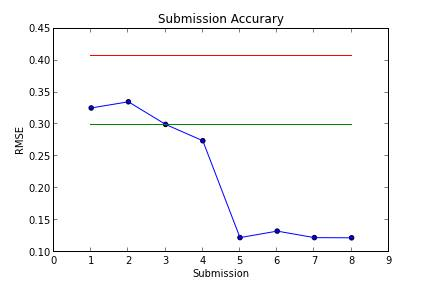
\includegraphics[scale=0.6]{accuracy_results}
\caption{Kaggle Scores in comparison to to baseline measurements. Note improvement from attempt 4 to attempt 5, marked by the critical creation of new features using RDkit.}
\label{fig:kaggle_score_two}
\end{figure}
\end{center}

\noindent The next approach in our results, as clearly highlighted by Figure \ref{fig:kaggle_score}, involved changing the method to the k-nearest neighbors. We had expected this to give us a large improvement over the last two attempts. However, as discussed in the above section, the results proved less than optimal. In particular, our hypothesis is that the reduction on features to a single dimension - due to the hardware limitations we faced - forced us to loose too much data. For this particular problem, is is our belief that attempting k-nearest neighbors would lead to results somewhere in the range of $0.15-0.20$. 
\begin{center}
\begin{figure}[h!]
\includegraphics[scale=0.2]{kaggle_score}
\caption{Full line graph demonstrating improvement over time with different models and feature sets. Critical breakthroughs are marked. Note that public and private scores match well, further corroborating the predictive ability of our model.}
\label{fig:kaggle_score}
\end{figure}  
\end{center}
\noindent Our final attempt using a large set of feature carefully extracted from the molecules proved more successful. In fact, the improvement is evident from both Figure \ref{fig:kaggle_score_two} and Figure \ref{fig:kaggle_score}. The large drop in RMS supports our hypothesis that the feature selection is of particular importance. The final set of attempts demonstrated in both graphs are simply variations on the number of components we reduced to using PCA. The reduction took place in order to decrease our computational requirements, but for the final submission, we again took advantage of the distributed system we had set-up and decided against PCA. Instead, we simply removed all features with zero-variance and trained on the remaining ($> 1800$). 

\noindent The sheer, massive increase in helpful features did not lead to the predicted improvement, likely due to the fact that we had already trained our model after  PCA reduction to $1024$ dimensions. It appears that at least some of the additional features extracted add little predictive potential to our model. Given the above results, we expect that computational resources can be further reduced through the removal of non-predictive or even highly correlated features. Furthermore, as discussed in the next section, it might be possible to continue development into the k-nearest neighbor algorithm. Now that great features have been selected, the next logical step is to return to the model selection in order to seek improvement in the RMS. 


\section{Further Development}
\subsection{Neural Networks}
Another promising model that we looked into was neural networks and deep learning. Neural networks are built upon a fundamental unit called sigmoid neurons, which takes in several inputs between 0 and 1 and produces a real-valued output. The sigmoid neuron has weights for every input, and the output is defined by the logistic function:
$$\sigma (z) = \frac{1}{1 + e^{-\sum_{i} w_i x_i - b}}$$
The simplest neural network would consist of 3 layers: inputs, hidden and output layers. We would employ the backpropagation algorithm to train the model. In the first phase of backpropagation, we would forward propagate the input values through randomly chosen weights to generate output activations, before back propagating in order to generate the errors of all output and hidden neurons. In the subsequent phase, we would obtain the gradient of the weight by multiplying the error and input activation, and subtract a multiple of that gradient from its previous weight. The multiple represents the learning rate.

\subsection{k-Nearest Neighbors Revisited}
For continued development, we would like to further narrow down our feature selection to the best possible features. If we can reduce it to 10 or so, it might be possible to run k-nearest neighbors on a home computer before graduating from Harvard.

\section{Conclusion}
Calculating the HOMO/LUMO gap for arbitrary molecules is a difficult and often computationally complex process. In this paper, we have explored different machine learning methods to predict the gap given the SMILES representation of a molecule. After several iterations through different models, we conclude with the following take-a-way: feature selection is one of the most important aspects in machine learning.\\
\\
\noindent The development complexity and large resource requirements of extracting extra features from the data is far outweighed by the huge potential benefit that selecting the correct subset of features for the model can have. Even with simple regression methods such as Lasso regression, the RMS improved by over $50\%$ when compared to the same method on worse features. In comparison, bad features led to little improvements even with more advanced methods. This conclusion makes intuitive sense - in any machine learning problem, the first few steps should focus on correct feature engineering. Once the features have been selected to a satisfactory level, the focus can shift to creating more complex models which can more accurately capture all of the implicit information present in the feature.

\onecolumn

\subsection{Large Figures}
Below we include additional figures as well as more detailed versions of the figures depicted in the above text.

\begin{center}
\begin{figure}[h!]
\includegraphics[scale=0.9]{covariance_plot}
\caption{Full plot of correlation plot showing intuitive covariances between non-zero variance features in the original data. Such correlation is indicative of linear dependence among these feature. Practically, this implies they would contribute little to the training of our model.}
\label{fig:correlation_plot_full}
\end{figure}

\begin{figure}[h!]
\includegraphics[angle=90,scale=0.65]{kaggle_score}
\caption{Full line graph demonstrating improvement over time with different models and feature sets. Critical breakthroughs are marked. Note that public and private scores match well, further corroborating the predictive ability of our mode.}
\label{fig:kaggle_score_full}
\end{figure}


\begin{figure}[h!]
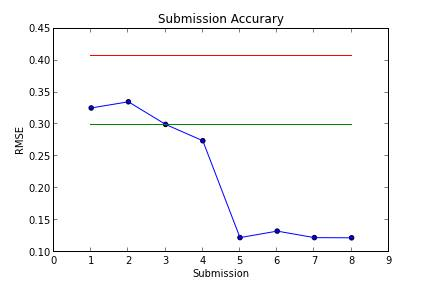
\includegraphics{accuracy_results}
\caption{Kaggle Scores in comparison to to baseline measurements. Note improvement from attempt 4 to attempt 5, marked by the critical creation of new features using RDkit.}
\label{fig:kaggle_score_two_full}
\end{figure}

\end{center}

\end{document}
























